\documentclass[12pt]{article}
\usepackage[dvipsnames]{xcolor}
\usepackage{times}
\usepackage[T1]{fontenc}
\usepackage{float}
\usepackage[margin=1.2in]{geometry}
\usepackage{graphicx}
\usepackage{textcomp}
\usepackage{titlesec}
\usepackage{enumitem}
\usepackage{adjustbox}
\usepackage{lastpage}
\usepackage{fancyvrb}

\graphicspath{ {./images/} }




\usepackage[colorlinks = true,
linkcolor = blue,
urlcolor  = blue,
citecolor = blue,
anchorcolor = blue]{hyperref}
\urlstyle{same}
\newcommand{\MYhref}[3][blue]{\href{#2}{\color{#1}{#3}}}%

% paragraphs are also numbered
\setcounter{secnumdepth}{3}
\titleformat{\paragraph}
{\normalfont\normalsize\bfseries}{\theparagraph}{1em}{}
\titlespacing*{\paragraph}
{0pt}{3.25ex plus 1ex minus .2ex}{1.5ex plus .2ex}

%No indent
\setlength{\parindent}{0pt}
\setenumerate{itemsep=0pt,parsep=0pt}


% https://en.wikibooks.org/wiki/LaTeX/Source_Code_Listings
\usepackage{listings, lstautogobble, beramono, tikz}

% Copy and paste text from boxes
\lstset{ 
	upquote=true,
	columns=fullflexible,
	basicstyle=\small\ttfamily,
	breaklines=true,
	postbreak=\mbox{\textcolor{red}{$\hookrightarrow$}\space},
	breakatwhitespace=false,
	backgroundcolor=\color{blue!20},
%	backgroundcolor=\color{black},
	showstringspaces=false,
	showspaces=false,    
	frameround=ffff,
	frame=single,
	rulecolor=\color{black},
	autogobble=true,
	literate={*}{{\char42}}1
	{-}{{\char45}}1
	{\ }{{\copyablespace}}1
}
\usepackage[space=true]{accsupp}
\newcommand{\copyablespace}{\BeginAccSupp{method=hex,unicode,ActualText=00A0}\hphantom{x}\EndAccSupp{}}

% Make boxes for code

\definecolor{mypink1}{rgb}{0.858, 0.188, 0.478}
% Highlight keywords
\lstset{
	emph=[1]{%  
		wget, gunzip, cd, docker,  grep, cut, sort, export%
	},emphstyle=[1]{\color{red}\bfseries},%
	emph=[2]{%  
		--mount, --workdir, -e%
	},emphstyle=[2]{\color{purple}\bfseries},%
	emph=[3]{%
		Salmo\_salar.ICSASG\_v2.dna.toplevel.fa.gz, Salmo\_salar.ICSASG\_v2.dna.toplevel.fa,  Salmo\_salar.ICSASG\_v2.dna.toplevel.fa.fai,
		Ssal\_chrm.txt
	},emphstyle=[3]{\color{blue}\bfseries},%
	emph=[4]{%  
		juettemann\/samtools:latest,  juettemann/genrich:0.6, alpine%
	},emphstyle=[4]{\color{Maroon}\bfseries},%
	emph=[5]{%  
		run, inspect, exec, pull, image, build, container, system, stop, kill	 
	},emphstyle=[5]{\color{brown}\bfseries},%
	emph=[6]{%  
		\$blast\_c
	},emphstyle=[6]{\color{TealBlue}\itshape},%
}%



\usepackage{fancyhdr}
\renewcommand{\headrulewidth}{.2mm} % header line width

\pagestyle{fancy}
\fancyhf{}
%\fancyhfoffset[L]{2cm} % left extra length
%\fancyhfoffset[R]{2cm} % right extra length
\rhead{\today}
\lhead{\bfseries ATAC-seq tutorial}
\rfoot{}
\rhead{
\includegraphics[width=1cm]{logo}}

\begin{document}
%	\begin{figure}[H]
%		
\includegraphics[scale=0.1]{logo.png}
%	\end{figure}
	
	% Article top matter
	\title{ATAC-seq} 
	\author{Thomas Juettemann, EMBL-EBI\\
		Lars Gr\o nvold, NMBU\\		
		\texttt{aqua\_faang\_course@ebi.ac.uk}}  %\texttt formats the text to a typewriter style font
	\date{May 10-12, 2021}  %\today is replaced with the current date
	\maketitle
	
	
	
	
	\section{Introduction}
	The aim of this section  is to investigate open chromatin regions in different tissues.  
	There are 4 sample replicates from brain (B), 4 from liver (L) and 4 from spleen (SP). 
	
	We are starting out with the BAM alignment files, which have been downloaded into the folder \textbf{train-aquafaang-bioinf/data} in the training home directory. The bam files are sorted by mapping position. Duplicates/multi-mapped reads and reads mapping to mitochondrial chromosome or unplaced scaffolds have been removed from all files.
	
	For simplicity, we are only processing replicate 1 from the brain samples. For the other sample replicates, all files have been made available in the respective folder.
	
	All processing is done using Docker with containerised applications. 

		\paragraph{Container}

			\begin{table}[H]
				\begin{center}
					\begin{adjustbox}{width=1\textwidth}
						\begin{tabular}{p{0.25\linewidth} | p{0.4\linewidth} | p{0.45\linewidth}}
							
							\multicolumn{1}{c}{ \textbf{Tool}} & \multicolumn{1}{c}{\textbf{Container}} & \multicolumn{1}{c}{\textbf{Documentation}} \\
							\hline
							samtools & \href{https://hub.docker.com/repository/docker/juettemann/samtools}{juettemann/samtools:latest} & \url{http://www.htslib.org/doc/sam.html} \\
							\hline
							Genrich & \href{https://hub.docker.com/repository/docker/juettemann/genrich}{juettemann/genrich:0.6} & \url{https://github.com/jsh58/Genrich}\\
							\hline
							bedgraphtobigwig & \href{https://quay.io/repository/biocontainers/ucsc-bedgraphtobigwig}{quay.io/biocontainers/ucsc-bedgraphtobigwig:377–h0b8a92\_2}- & \url{https://genome.ucsc.edu/goldenPath/help/bigWig.html#Ex3}\\
							\hline
							ataqv & \href{https://quay.io/repository/biocontainers/ataqv?tag=1.2.1-py27h97b49fa_1}{quay.io/biocontainers/ataqv:1.2.1
								–py27h97b49fa\_1} & \url{https://github.com/juettemann/ataqv/tree/patch-1} \\
							\hline
						\end{tabular}
					\end{adjustbox}
					\caption[Container]{Container used in this tutorial }
					\label{table:genrich}
				\end{center}
			\end{table}

	\paragraph{File formats}
			
		\begin{table}[H]
			\begin{center}
				\begin{adjustbox}{width=1\textwidth}
					\begin{tabular}{p{0.15\linewidth} | p{0.4\linewidth} | p{0.5\linewidth}}

						\multicolumn{1}{c}{ \textbf{Extension}} & \multicolumn{1}{c}{\textbf{Description}} & \multicolumn{1}{c}{\textbf{Documentation}} \\
						\hline
						sam & Sequence Alignment/Map file format &\url{http://www.htslib.org/doc/sam.html} \\
						\hline
						bam & Binary Format of Sequence Alignment/Mapping (SAM) & \url{https://genome.ucsc.edu/ENCODE/fileFormats.html#BAM}\\
						\hline
						bigWig & Genome Browser Signal (Wiggle) Files in Indexed Binary Format & \url{https://genome.ucsc.edu/ENCODE/fileFormats.html#bigWig}\\
						\hline
						narrowPeak & ENCODE narrowPeak: Narrow (or Point-Source) Peaks format& \url{https://genome.ucsc.edu/FAQ/FAQformat.html#format12}  \\
						\hline
						faidx & An index enabling random access to FASTA and FASTQ files & \url{http://www.htslib.org/doc/faidx.html} \\
						\hline 
					\end{tabular}
				\end{adjustbox}
				\caption[FileFormats]{File formats used in this tutorial }
				\label{table:genrich}
			\end{center}
		\end{table}
	

	
	\section{Variables}
	In order to make commands shorter and allow less chance for errors, we are setting a few  environment variables. These have already been set in the .bashrc.
	
	\vspace{0.5cm}	
	\begin{minipage}{\linewidth}
		\begin{lstlisting}
			export dir_atac="$HOME/train-aquafaang-bioinf/atac-seq"
			export mnt_dir_atac="type=bind,source=$dir_atac,target=/mnt"
		\end{lstlisting}
	\end{minipage}

	\section{Reference Genome}
		Like other *-seq experiments, also ATAC-seq relies on a reference genome
		We will be using the \textit{ International Cooperation to Sequence the Atlantic Salmon Genome  version 2 (ICSASG\_v2)} genome from 2015 for this course. 
		General information about the assembly can be found at Ensembl (\url{https://www.ensembl.org/Salmo_salar/Info/Index}).
		On that page you also find links to FASTA files with the DNA sequence (reference genome) and gtf files with the Ensembl gene annotation.
		
		\subsection{Download}
			Your first task is to find, download and unzip the atlantic salmon reference sequence
			
			\paragraph{Task}
			
				\fcolorbox{black}[HTML]{E9F0E9}{\parbox{\linewidth}{%	
					\begin{enumerate}
						\item Open a terminal
						\item Change directory to \textbf{\$dir\_atac/ref\_genome}.
						\item On the Ensembl assembly page, find the DNA sequence in FASTA format.
						\item Click on the link (you will be redirected to a FTP directory).
						\item Locate  \textbf{toplevel}  FASTA file (.fa).
						\item Right-click on it and choose \textit{Copy Link Location}
						\item In the terminal, download the file using \textit{wget}
						\item Unzip (\textit{gunzip})
					\end{enumerate}
				}}
			
			\paragraph{Solution}
			
			%	\vspace{0.5cm}	
				\begin{minipage}{\linewidth}
					\begin{lstlisting}
						cd $dir_atac/ref_genome  
						wget http://ftp.ensembl.org/pub/release-103/fasta/salmo_salar/dna/Salmo_salar.ICSASG_v2.dna.toplevel.fa.gz
						gunzip Salmo_salar.ICSASG_v2.dna.toplevel.fa.gz
					\end{lstlisting}
				\end{minipage}
		
		
		\subsection{Create FASTA index}
			Using an fai index file in conjunction with a FASTA  file containing reference sequences enables efficient access to arbitrary regions within those reference sequences. 
			The index file typically has the same filename as the corresponding FASTA, with .fai appended.
			An fai index file is a text file consisting of lines each with five TAB-delimited columns for a FASTA file:
			\begin{enumerate}
				\item NAME	Name of this reference sequence
				\item LENGTH	Total length of this reference sequence, in bases
				\item OFFSET	Offset in the FASTA/FASTQ file of this sequence's first base
				\item LINEBASES	The number of bases on each line
				\item LINEWIDTH	The number of bytes in each line, including the newline
			\end{enumerate}
		
			Using a samtools container, index the fasta file (\textit{Salmo\_salar.ICSASG\_v2.dna.toplevel.fa}). 
			This resulting index file's name should be \textit{Salmo\_salar.ICSASG\_v2.dna.toplevel.fa.fai}
		
			\paragraph{Task}
				\fcolorbox{black}[HTML]{E9F0E9}{\parbox{\linewidth}{%	
						\begin{enumerate}
							\item Pull the container\textbf{ juettemann/samtools:latest} \\
							(Documentation: \url{http://www.htslib.org/doc/samtools-faidx.html})
							\item Using  \textbf{faidx} from the container, index \textit{Salmo\_salar.ICSASG\_v2.dna.toplevel.fa}
						\end{enumerate}
				}}
		
			\paragraph{Solution}
			
				\begin{minipage}{\linewidth}
					\begin{lstlisting}
						# docker run pulls the container automatically if not available
						docker run --mount $mnt_dir_atac juettemann/samtools:latest faidx /mnt/ref_genome/Salmo_salar.ICSASG_v2.dna.toplevel.fa
					\end{lstlisting}
				\end{minipage}
		
		\subsection{Create list of chromosomes}	
			At a later stage in the tutorial, we need a list of all autosomal chromosomes. 
			Using the command line utilities grep and cut, create a file containing only the chromosome names. 
			As mentioned above in the faidx description, the name of the reference sequence is the first column in the FASTA index file, and chromosomes start with \textit{ssa}.

			\paragraph{Task}
		
				\fcolorbox{black}[HTML]{E9F0E9}{\parbox{\linewidth}{%	
						\begin{enumerate}
							\item Using \textbf{grep} and \textbf{cut}, extract all chromosome names
							\item Store the names in in the \textbf{\$dir\_atac/ref\_genome} folder in a file named \textbf{Ssal\_chrm.txt}
						\end{enumerate}
				}}
			
			\paragraph{Solution}
			
				\begin{minipage}{\linewidth}
					\begin{lstlisting}
						cd $dir_atac/ref_genome/
						grep ^ssa Salmo_salar.ICSASG_v2.dna.toplevel.fa.fai | cut -f 1 > Ssal_chrm.txt
					\end{lstlisting}
				\end{minipage}
		
		\subsection{Create table with chromosome sizes}
			We will be converting bedgraph files to bigWig later. 
			For that conversion, we need a file containing chromosome name and its size. 
			We already know that the chromosome name is the first column, and looking at the description of samtools faidx above, we see that the length is stored in the second column.
			 
			\paragraph{Task}
			
			\fcolorbox{black}[HTML]{E9F0E9}{\parbox{\linewidth}{%	
					\begin{enumerate}
						\item Using \textbf{grep} and \textbf{cut}, extract all chromosome names and their length.
						\item Store the names in the \textbf{\$dir\_atac/ref\_genome} folder in a file named \textbf{Ssal\_chrm\_sizes.txt}
					\end{enumerate}
			}}
			
			\paragraph{Solution}
			
				\begin{minipage}{\linewidth}
					\begin{lstlisting}
						cd $dir_atac/ref_genome/
						grep ^ssa Salmo_salar.ICSASG_v2.dna.toplevel.fa.fai | cut -f 1,2 >Ssal_chrm_sizes.txt
					\end{lstlisting}
				\end{minipage}
	
	\section{Peak Calling} 
		The tool we are using for peak calling is Genrich. Genrich was  developed by John Gaspar, previous of Harvard FAS Informatics. 
		The default method is for ChIP-seq peak-calling, but there is an ATAC-seq specific mode. 
		To account for the manner in which the Tn5 enzyme inserts itself into the genome, Genrich centers a 100 bp interval at each end of each fragment. 
		It uses the log-normal distribution to calculate p-values for each base of the genome.
		
		Some advantages over MACS include how much faster it runs (it is written in C), as well as the capability of calling peaks for multiple replicates collectively. 
		Unfortunately, Genrich is yet to be published.
		
		\subsection{Sort by read names}
			Genrich requires that the BAM files are sorted by read names, not by mapping position, which they currently are.
			
			Sort bam file by reads, name it \textit{B-1.sortedByRead.bam} and store it in \textit{results/genrich/}. Samtools documentation: \url{http://www.htslib.org/doc/samtools.html}	
			
			\paragraph{Task}
			
				\fcolorbox{black}[HTML]{E9F0E9}{\parbox{\linewidth}{%	
						\begin{enumerate}
							\item Using the \textbf{ juettemann/samtools:latest} container \textbf{sort} \$dir\_atac/data/B-1.bam by read names\\
							(Documentation \url{http://www.htslib.org/doc/samtools-sort.html})
							\item Name the output file \textbf{B-1.sortedByRead.bam} and store it in the folder \textbf{\$dir\_atac/results/genrich/} 
							\item Set number of sorting and compression threads to 8
						\end{enumerate}
				}}
			
			\paragraph{Solution}
				
				\begin{minipage}{\linewidth}
					\begin{lstlisting}
						docker run \
						--mount $mnt_dir_atac \
						juettemann/samtools:latest sort -n -@ 8 -o /mnt/results/genrich/B-1.sortedByRead.bam /mnt/data/B-1.bam	
					\end{lstlisting}
				\end{minipage}
		
		\subsection{Peak calling}
			Next step is the peak calling with Genrich. 
			
			\paragraph{Task}
			
			\fcolorbox{black}[HTML]{E9F0E9}{\parbox{\linewidth}{%	
					\begin{enumerate}
						\item  Pull the container  \textbf{juettemann/genrich:1.0} \\
						(Documentation  \url{https://github.com/jsh58/Genrich})
						\item Using\textbf{ \$dir\_atac/results/genrich/B-1.sortedByRead.bam} as input, create:
						\begin{itemize}
							\item ENCODE narrowPeak format
							\item bedgraph-ish file for pileups and p-values
							\item Set:
							\begin{itemize}
								\item Maximum q-value = 0.05
								\item print status to stderr
								\item ATAC-seq mode 
							\end{itemize}
							\item Redirect the STDERR output to \textbf{\$dir\_atac/logs/genrich\_B-1.log}
						\end{itemize}
					\end{enumerate}
			}}
			
			
			\paragraph{Solution}
				
			\begin{minipage}{\linewidth}
				\begin{lstlisting}
					docker run --mount $mnt_dir_atac juettemann/genrich:0.6 -t  /mnt/results/genrich/B-1.sortedByRead.bam -o /mnt/results/genrich/B-1.narrowPeak -k /mnt/results/genrich/B-1.k.bedGraph -q 0.05 -v -j 2> $dir_atac/logs/genrich_B-1.log
				\end{lstlisting}
			\end{minipage}
	
	\section{Quality Control}
		We will be using two tools for investigating the results of the peak calling, Integrated Genome Browser (IGV) and ataqv.
		
		\subsection{IGV}
			A common way to get an idea about the quality of the results is looking at the data in a genome browser. 
			As most publicly available web based browsers have a limit on the size of the file that you can upload, we will be using IGV.
			Visualising the read density along the chromosomes (bigwig files) and the peaks defined by Genrich(narrowPeak file).
		
			\subsubsection{Convert bedGraph to BigWig}
				The bigWig format is for display of dense, continuous data that will be displayed as a graph. 
				The main advantage of the bigWig files is that only the portions of the files needed to display a particular region are transferred, so for large data sets bigWig is considerably faster than any non-indexed formats.


			\paragraph{Create compliant bedGraph }
				The  .bedGraph-ish out from Genrich can easily be converted to bigWig. 
				To create a compliant bedGraph file, extra columns and headers must be removed. 
				
				\paragraph{Task}
					
					\fcolorbox{black}[HTML]{E9F0E9}{\parbox{\linewidth}{%	
						\begin{enumerate}
							\item Using \textbf{grep} and \textbf{cut}, extract all chromosome names and columns 1-4
							\item Store the names in the \textbf{\$dir\_atac/results/genrich/} folder in a file named \textbf{B-1.k.fixed.bedGraph}
						\end{enumerate}
					}}
				
				\paragraph{Solution}
					
					\begin{minipage}{\linewidth}
						\begin{lstlisting}
							cd $dir_atac/results/genrich/
							grep ^ssa B-1.k.bedGraph | cut -f 1-4 > B-1.k.fixed.bedGraph
						\end{lstlisting}
					\end{minipage}
					
					
			\paragraph{Create bigWig}
					UCSC provides a tool to convert bedGraph to bigWig (part of the Kent tools). It takes 3 arguments:\\
					
					 \textbf{bedGraphToBigWig} <i\textit{in.bedGraph}> <\textit{chrom.sizes}> <\textit{outBigWig.bw}>\\
				
					
				\paragraph{Task}

					\fcolorbox{black}[HTML]{E9F0E9}{\parbox{\linewidth}{%	
							\begin{enumerate}
								\item  Using \textbf{quay.io/biocontainers/ucsc-bedgraphtobigwig:377--h0b8a92\_2}, convert \textbf{B-1.k.fixed.bedGraph} to \textbf{B-1.bw}
								\item  Save the file in \textbf{\$dir\_atac/results/genrich/}
							\end{enumerate}
					}}
					
					\paragraph{Solution}
	
					\begin{minipage}{\linewidth}
						\begin{lstlisting}
							docker run --mount $mnt_dir_atac quay.io/biocontainers/ucsc-bedgraphtobigwig:377--h0b8a92a_2 bedGraphToBigWig /mnt/results/genrich/B-1.k.fixed.bedGraph /mnt/ref_genome/Ssal_chrm_sizes.txt /mnt/results/genrich/B-1.bw
						\end{lstlisting}
					\end{minipage}
		
		\subsubsection{Launch IGV}
			The IGV browser is launched from the command line. 
			
				\paragraph{Task}
			
			\fcolorbox{black}[HTML]{E9F0E9}{\parbox{\linewidth}{%	
					\begin{enumerate}
						\item  Open a new terminal and run
						\item  igv
					\end{enumerate}
			}}
			
			
		\subsubsection{Load Genome and Tracks}
			IGV loads its genomes from the Broad Institute, and these genomes use RefSeq accessions as chromosome names. 
			Refseq accessions are different from the ones used by the submitter of the genome (which Ensembl uses), therefore we need to load this standard genome manually.
			
			\paragraph{Task}
			
				\fcolorbox{black}[HTML]{E9F0E9}{\parbox{\linewidth}{%	
					\begin{enumerate}
						\item In the IGV window, click \textit{Genomes} -> \textit{Load Genome from File} -> navigate to  \textit{train-aquafaang-bioinf/atac-seq/ref\_genome/} and select \\
						-> \textbf{Salmo\_salar.ICSASG\_v2.dna.toplevel.fa} 
						\item In the IGV window, click \textit{File} -> \textit{Load from File} -> navigate to \textit{train-aquafaang-bioinf/atac-seq/results/genrich/} and select\\
						-> \textit{Salmo\_salar.ICSASG\_v2.103.chr.sorted.gtf}
						-> \textit{B-1.bw} \\
						-> \textit{B-1.narrowPeak} \\
						-> \textit{L-1.bw} \\
						-> \textit{L-1.narrowPeak}
					\end{enumerate}
				}}
		
		If you want to go futher and  get an idea about the differences between the replicates, simply load all other *.bw and *.narrowPeak files the same way.
		
		\subsubsection{Explore using IGV}
			We will investigate two genes, \textit{Neurogenic differentiation factor} (\textbf{NDF1}) which is involved in neuron development, and \textit{Hepatocyte nuclear factor 1-alpha} (\textbf{hnf1a}) which is involved in liver development. 
			
			\paragraph{NDF1}
			The genomic coordinates of NDF1 are  \textit{ssa25:27,019,821-27,030,126}. Copy and paste them in the seach box and click Go. 
			Figure \ref{fig:ndf1} shows the expected result. 
			The sample B-1 has open chromatin upstream of the NDF1 gene (peak\_59291), whereby the liver samples show closed chromatin.   
			
			\begin{figure}[H]
				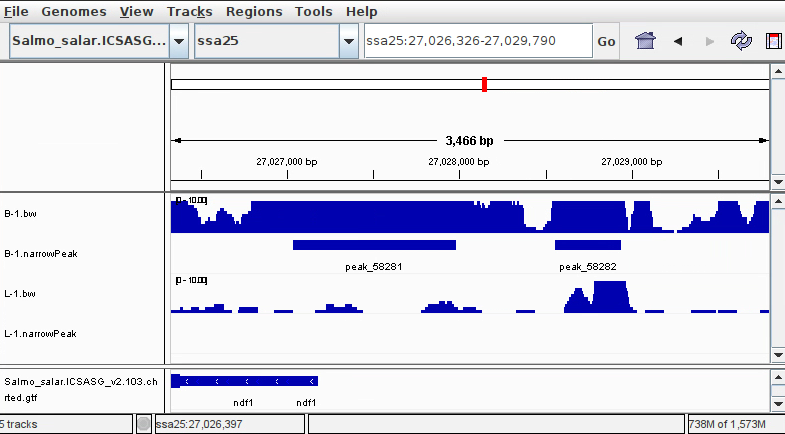
\includegraphics[width=\textwidth]{ndf1.png}
				\caption{IGV showing area around the NDF1 gene}
				\label{fig:ndf1}	
			\end{figure}
			
			\paragraph{hnf1a}
			The genomic coordinates of hnf1a are  \textit{ssa20:19,522,855-19,530,228}. 
			Copy and paste them in the search box and click Go. 
			In figure \ref{fig:hnf1a}, the roles are reversed - the liver sample shows open chromatin upstream of the hnf1a gene (peak\_51067).
		
			\begin{figure}[H]
				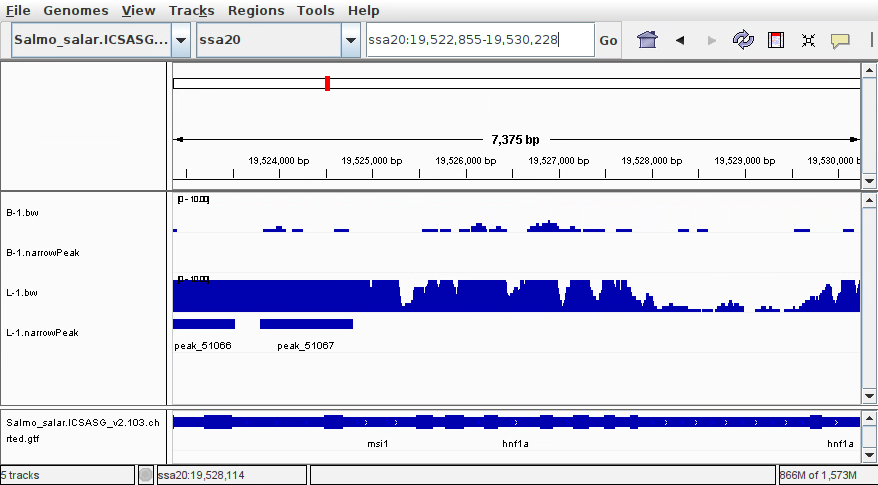
\includegraphics[width=\textwidth]{hnf1a.png}
				\caption{IGV showing area around the hnf1a gene}
				\label{fig:hnf1a}		
			\end{figure}
			
			The overlap between the msi1 gene and hnf1a can easily be explained by having a look at the Ensembl genome browser (figure \ref{fig:msi1}), the last intron of transcript 202 extends into hnf1.
			
			\begin{figure}[H]
				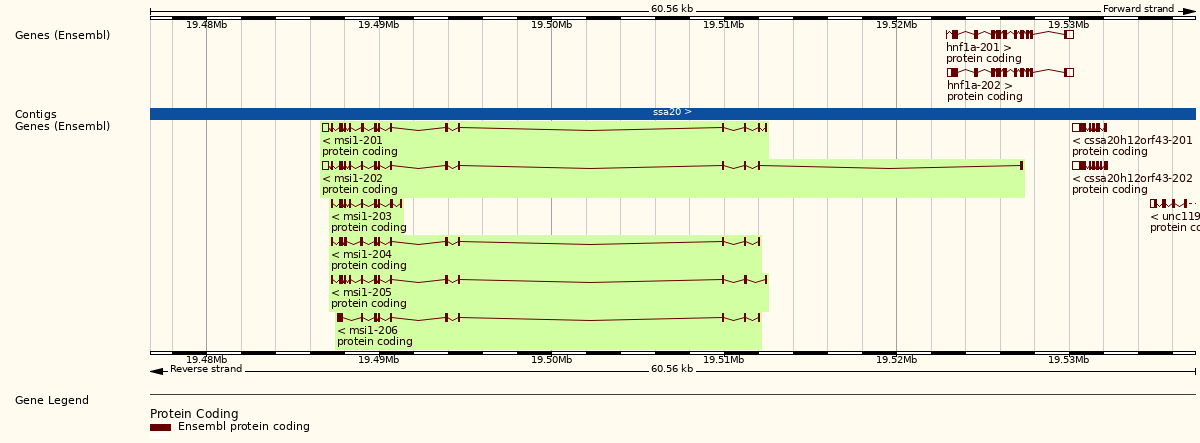
\includegraphics[width=\textwidth]{Atlantic_salmon_msi1.png}
				\caption{msi1 gene in the Ensembl genome browser}
				\label{fig:msi1}
			\end{figure}
		
		\subsection{ATAQV}
			Ataqv is a toolkit for measuring and comparing a broad range of ATAC-seq quality metrics. 
			It makes it easier to spot differences that might be caused by library prep or sequencing. 
			We will investigate two features: high quality autosomal alignment (HQAA) fragment length distribution (FLD) and  transcription start sites (TSS) enrichment.
		
		\subsubsection{Index BAM}
			To run ATAQV the BAM file needs to be indexed. 
			Using samtools, index B-1.bam.
			
			\paragraph{Task}
			
				\fcolorbox{black}[HTML]{E9F0E9}{\parbox{\linewidth}{%	
						\begin{enumerate}
							\item  Using \textbf{ juettemann/samtools} index, convert \textbf{\$dir\_atac/data/B-1.bam} to \textbf{B-1.bw}
							\item  Name the output \textbf{B-1.bam.bai} and save the file in \textbf{\$dir\_atac/data}
						\end{enumerate}
				}}
			
			\paragraph{Solution}
				\begin{minipage}{\linewidth}
					\begin{lstlisting}
						docker run --mount $mnt_dir_atac juettemann/samtools index /mnt/data/B-1.bam /mntdata/B-1.bam.bai
					\end{lstlisting}
				\end{minipage}
		
		\subsubsection{Run ATAQV}
			The main program, ataqv, examines our aligned reads and reports some basic metrics.
			
%			\begin{enumerate}
%				\item reads mapped in proper pairs
%				\item optical or PCR duplicates
%				\item reads mapping to autosomal or mitochondrial references
%				\item the ratio of short to mononucleosomal fragment counts
%				\item mapping quality
%				\item various kinds of problematic alignments
%			\end{enumerate}
%			If you also have a file of peaks called on your data, that file can be examined to report read coverage of the peaks.
%			With a file of transcription start sites, ataqv can report a TSS enrichment metric based on the transposition activity around those locations.
%			The report is printed as plain text to standard output, and detailed metrics are written to JSON files for further processing.
%			
%			
%			The chromosome names of our genome are non-standard as they start with "ssa". Standard (autosomal) chromosome names are either chr1 or 1.
%			ataqv has an option, --autosomal-reference-file:
%			"A file containing autosomal reference names, one per line. The names must match the reference names in the alignment file exactly, or the metrics based on counts of autosomal alignments will be wrong." 
%			The bed file for TSS enrichment has been created already and placed in the \$atac\_dir/ref\_genome folder.	 
%			Documentation: \url{https://github.com/ParkerLab/ataqv}
			
			\paragraph{Task}
			
			\fcolorbox{black}[HTML]{E9F0E9}{\parbox{\linewidth}{%	
					\begin{enumerate}
						\item  Using \textbf{quay.io/biocontainers/ataqv:1.2.1--py27h97b49fa\_1 ataqv} run \textbf{ataqv}\\
						(Documentation: \url{https://github.com/ParkerLab/ataqv})
						\item ataqv needs information about our terminal, pass \textbf{-e TERM=xterm} to the container.
						\item Input
						\begin{itemize}
							\item organism name is Ssal
							\item alignment file \$dir\_atac/data/B-1.bam
							\item peak file is \$dir\_atac/results/genrich/B-1.narrowPeak
							\item TSS file is \$dir\_atac//ref\_genome/SsalTSS\_NCBI.bed
							\item autosomal reference is \$dir\_atac//ref\_genome/Ssal\_chrm.txt
						\end{itemize}
						\item Output
							\begin{itemize}
								\item metrics file 	 \$dir\_atac/results/ataqv/B-1.ataqv.json
							\end{itemize}
					\end{enumerate}
			}}
			
			\paragraph{Solution}
			
			\begin{minipage}{\linewidth}
				\begin{lstlisting}
					docker run -e  TERM=xterm  --mount $mnt_dir_atac quay.io/biocontainers/ataqv:1.2.1--py27h97b49fa_1 	ataqv  Ssal  /mnt/data/B-1.bam --peak-file /mnt/results/genrich/B-1.narrowPeak 	--tss-file /mnt/ref_genome/SsalTSS_NCBI.bed --autosomal-reference-file /mnt/ref_genome/Ssal_chrm.txt --metrics-file /mnt/results/ataqv/B-1.ataqv.json
				\end{lstlisting}
			\end{minipage}
			
		\subsubsection{Visualising results}
			The mkarv script that collects ataqv results and sets up a web application to visualize them.
			
			\paragraph{Task}
			
				\fcolorbox{black}[HTML]{E9F0E9}{\parbox{\linewidth}{%	
						\begin{enumerate}
						\item  Using \textbf{quay.io/biocontainers/ataqv:1.2.1--py27h97b49fa\_1 ataqv} run \textbf{mkarv}\\
						(Documentation: \url{https://github.com/ParkerLab/ataqv})
						\item  Pass \textbf{-e TERM=xterm} to the container.
						\item Input
						\begin{itemize}
							\item results/mkarv/ataqv\_good\_html 
							\item whitespace separated list of all 8 B \& L *.ataqv.json files, e.g.  \textbf{results/ataqv/B-1.ataqv.json}  
						\end{itemize}
						\end{enumerate}
				}}
			
			\paragraph{Solution}
				
				\begin{minipage}{\linewidth}
					\begin{lstlisting}
						docker run -e  TERM=xterm --mount $mnt_dir_atac quay.io/biocontainers/ataqv:1.2.1--py27h97b49fa_1 mkarv  /mnt/results/mkarv/ataqv_good_html /mnt/results/ataqv/B-1.ataqv.json /mnt/results/ataqv/B-2.ataqv.json /mnt/results/ataqv/B-3.ataqv.json /mnt/results/ataqv/B-4.ataqv.json /mnt/results/ataqv/L-1.ataqv.json /mnt/results/ataqv/L-2.ataqv.json /mnt/results/ataqv/L-3.ataqv.json /mnt/results/ataqv/L-4.ataqv.json
					\end{lstlisting}
				\end{minipage}
			
			Now we do the same for the spleen samples.
			
			\paragraph{Task}
			
			\fcolorbox{black}[HTML]{E9F0E9}{\parbox{\linewidth}{%	
					\begin{enumerate}
						\item  Using \textbf{quay.io/biocontainers/ataqv:1.2.1--py27h97b49fa\_1 ataqv} run \textbf{mkarv}\\
						(Documentation: \url{https://github.com/ParkerLab/ataqv})
						\item  Pass \textbf{-e TERM=xterm} to the container.
						\item Input
						\begin{itemize}
							\item results/mkarv/ataqv\_bad\_html 
							\item whitespace separated list of all 4 SP *.ataqv.json files, e.g.  \textbf{results/ataqv/SP-1.ataqv.json}  
						\end{itemize}
					\end{enumerate}
			}}
			
			\paragraph{Solution}	
			
			\begin{minipage}{\linewidth}
				\begin{lstlisting}
					docker run  -e  TERM=xterm --mount $mnt_dir_atac quay.io/biocontainers/ataqv:1.2.1--py27h97b49fa_1  mkarv /mnt/results/mkarv/ataqv_bad_html /mnt/results/ataqv/SP-1.ataqv.json /mnt/results/ataqv/SP-2.ataqv.json /mnt/results/ataqv/SP-3.ataqv.json /mnt/results/ataqv/SP-4.ataqv.json
				\end{lstlisting}
			\end{minipage}
			
			In your webbrowser, navigate to directory \$dir\_atac/results/markv/ataqv\_good\_html  and  open the index html. 
			Explore the different graphs and also the table tab.
			
			\begin{figure}[H]
				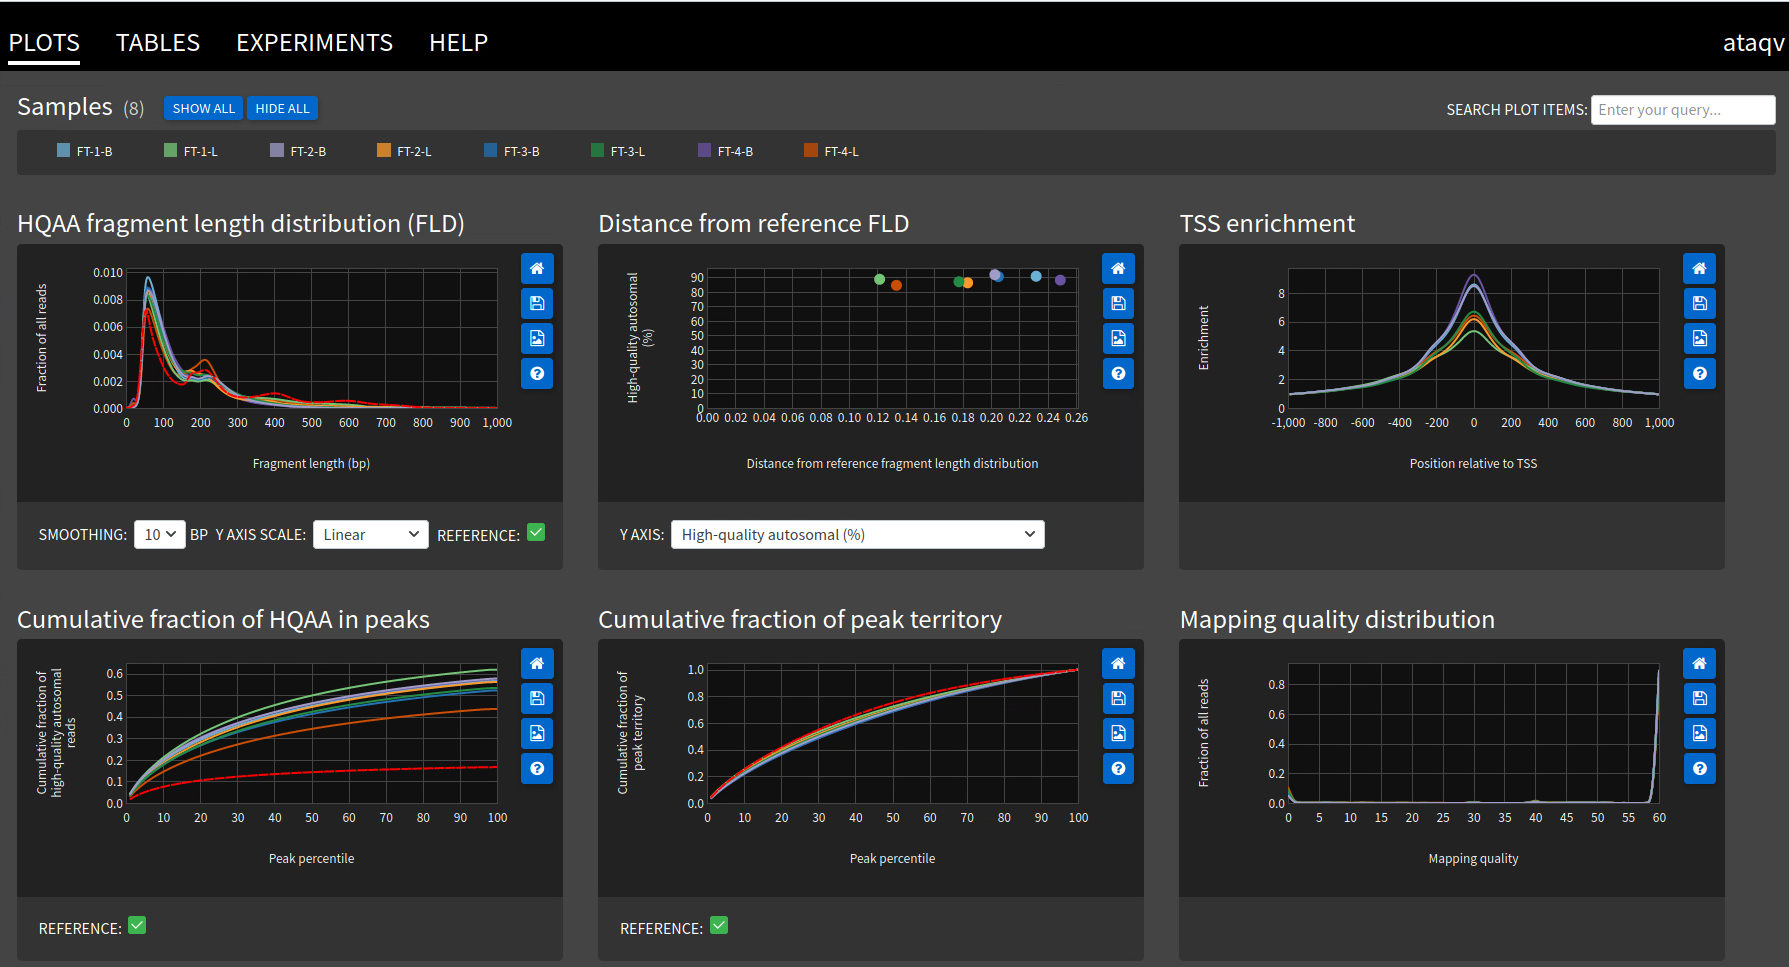
\includegraphics[width=\textwidth]{ataqv_good.png}
				\caption{Result of a successful  ATAC-seq experiment visualised using ataqv}
				\label{fig:ataqv_good}
			\end{figure}
			
			Now do the same for spleen sample results (\$dir\_atac/results/markv/ataqv\_good\_html/index.html). 
			What differences do you see?
			
			\begin{figure}[H]
				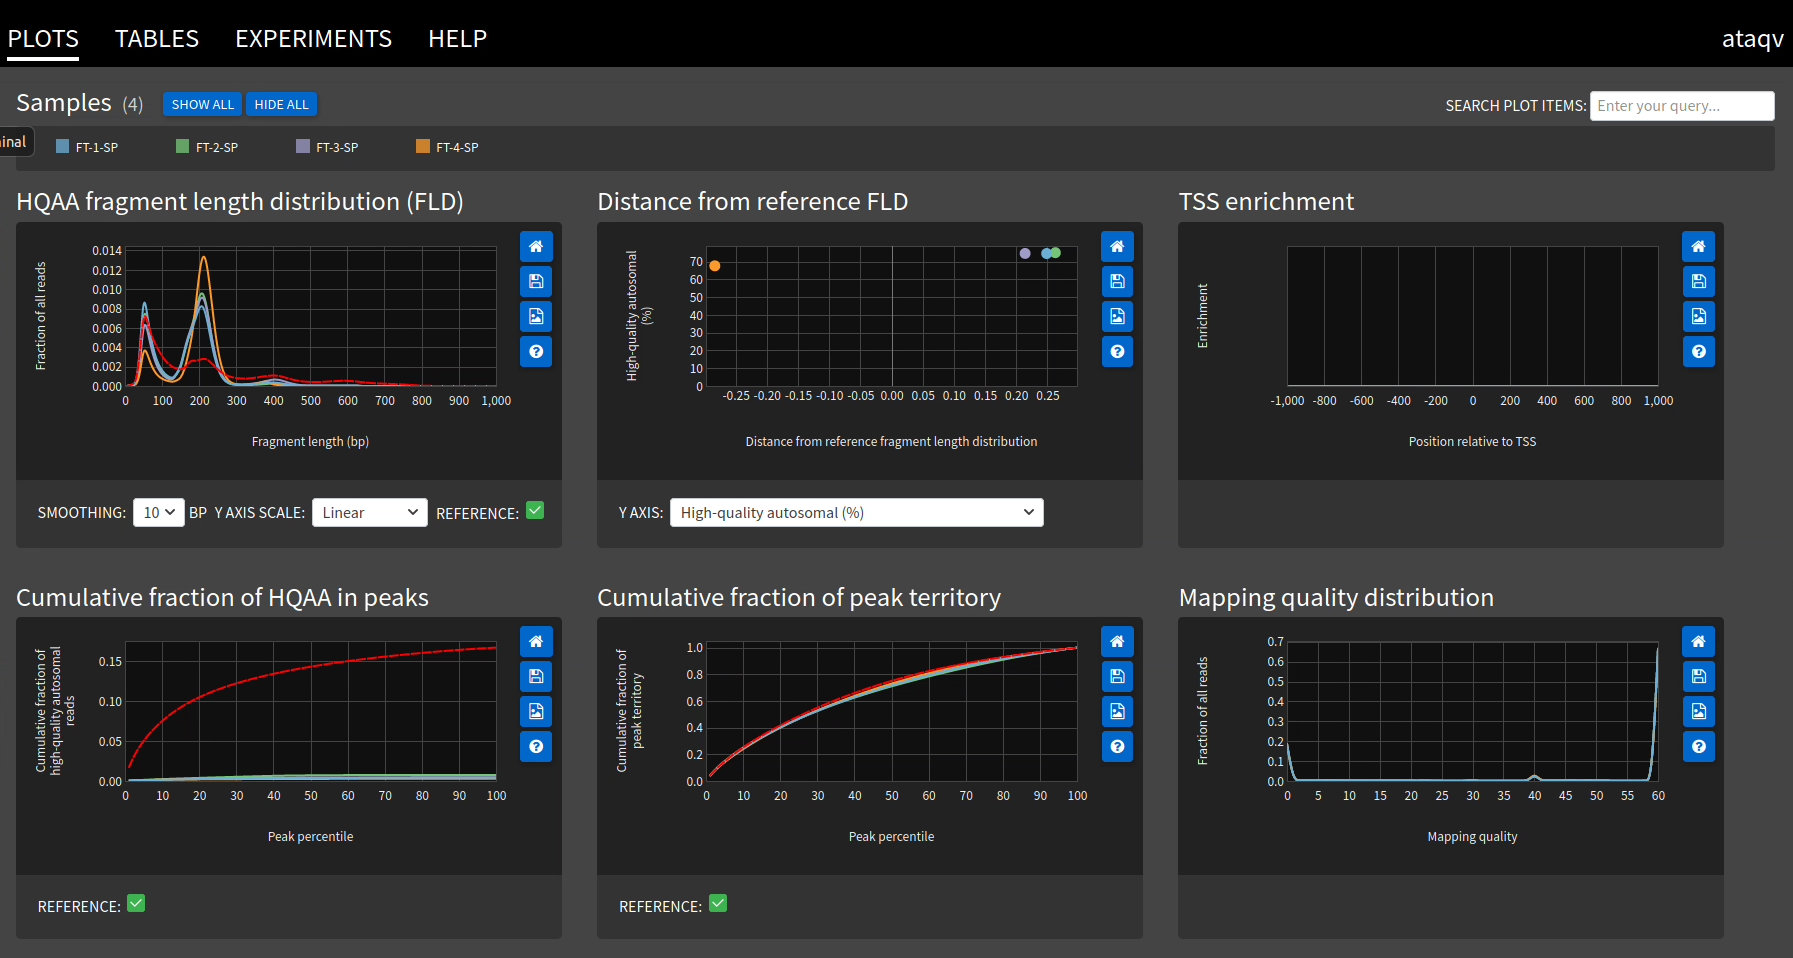
\includegraphics[width=\textwidth]{ataqv_bad.png}
				\caption{Result of an unsuccessful  ATAC-seq experiment visualised using ataqv}
				\label{fig:ataqv_bad}
			\end{figure}
	

	
\end{document}  %End of document.